\documentclass[12pt,a4paper]{scrreprt}
 \usepackage{ngerman}
 \usepackage[utf8]{inputenc}

\usepackage{listings}


 \usepackage[T1]{fontenc}
\usepackage{pdfpages}
\usepackage{url}
\graphicspath{{/Users/Timo/Documents/DHBW/Semester4/Projektarbeit/}}
\usepackage{graphicx}
\usepackage{wrapfig}
\usepackage{geometry} 
\geometry{a4paper, top=25mm, left=25mm, right=25mm, bottom=25mm, headsep=15mm, 
  footskip=12mm}
\usepackage{textcomp}
% Header
\usepackage{fancyhdr}
\pagestyle{fancy}
% Header für Seiten ohne Chapter
\fancyhf{}
\fancyhead[L]{Studienarbeit Timo Höting \\ DHBW Karlsruhe}
   \fancyhead[R]{
\includegraphics[scale=0.3]{./data/dhbwlogo.jpg} } 
\fancyfoot[C]{\thepage}
\fancypagestyle{plain}{
% Header für Seiten mit Chapter
\fancyhf{}
   \fancyhead[L]{Studienarbeit Timo Höting \\ DHBW Karlsruhe}
   \fancyhead[R]{
\includegraphics[scale=0.3]{./data/dhbwlogo.jpg} } 
\fancyfoot[C]{\thepage}
}

 \begin{document}
\begin{titlepage}
\begin{figure}
\makebox[\textwidth]{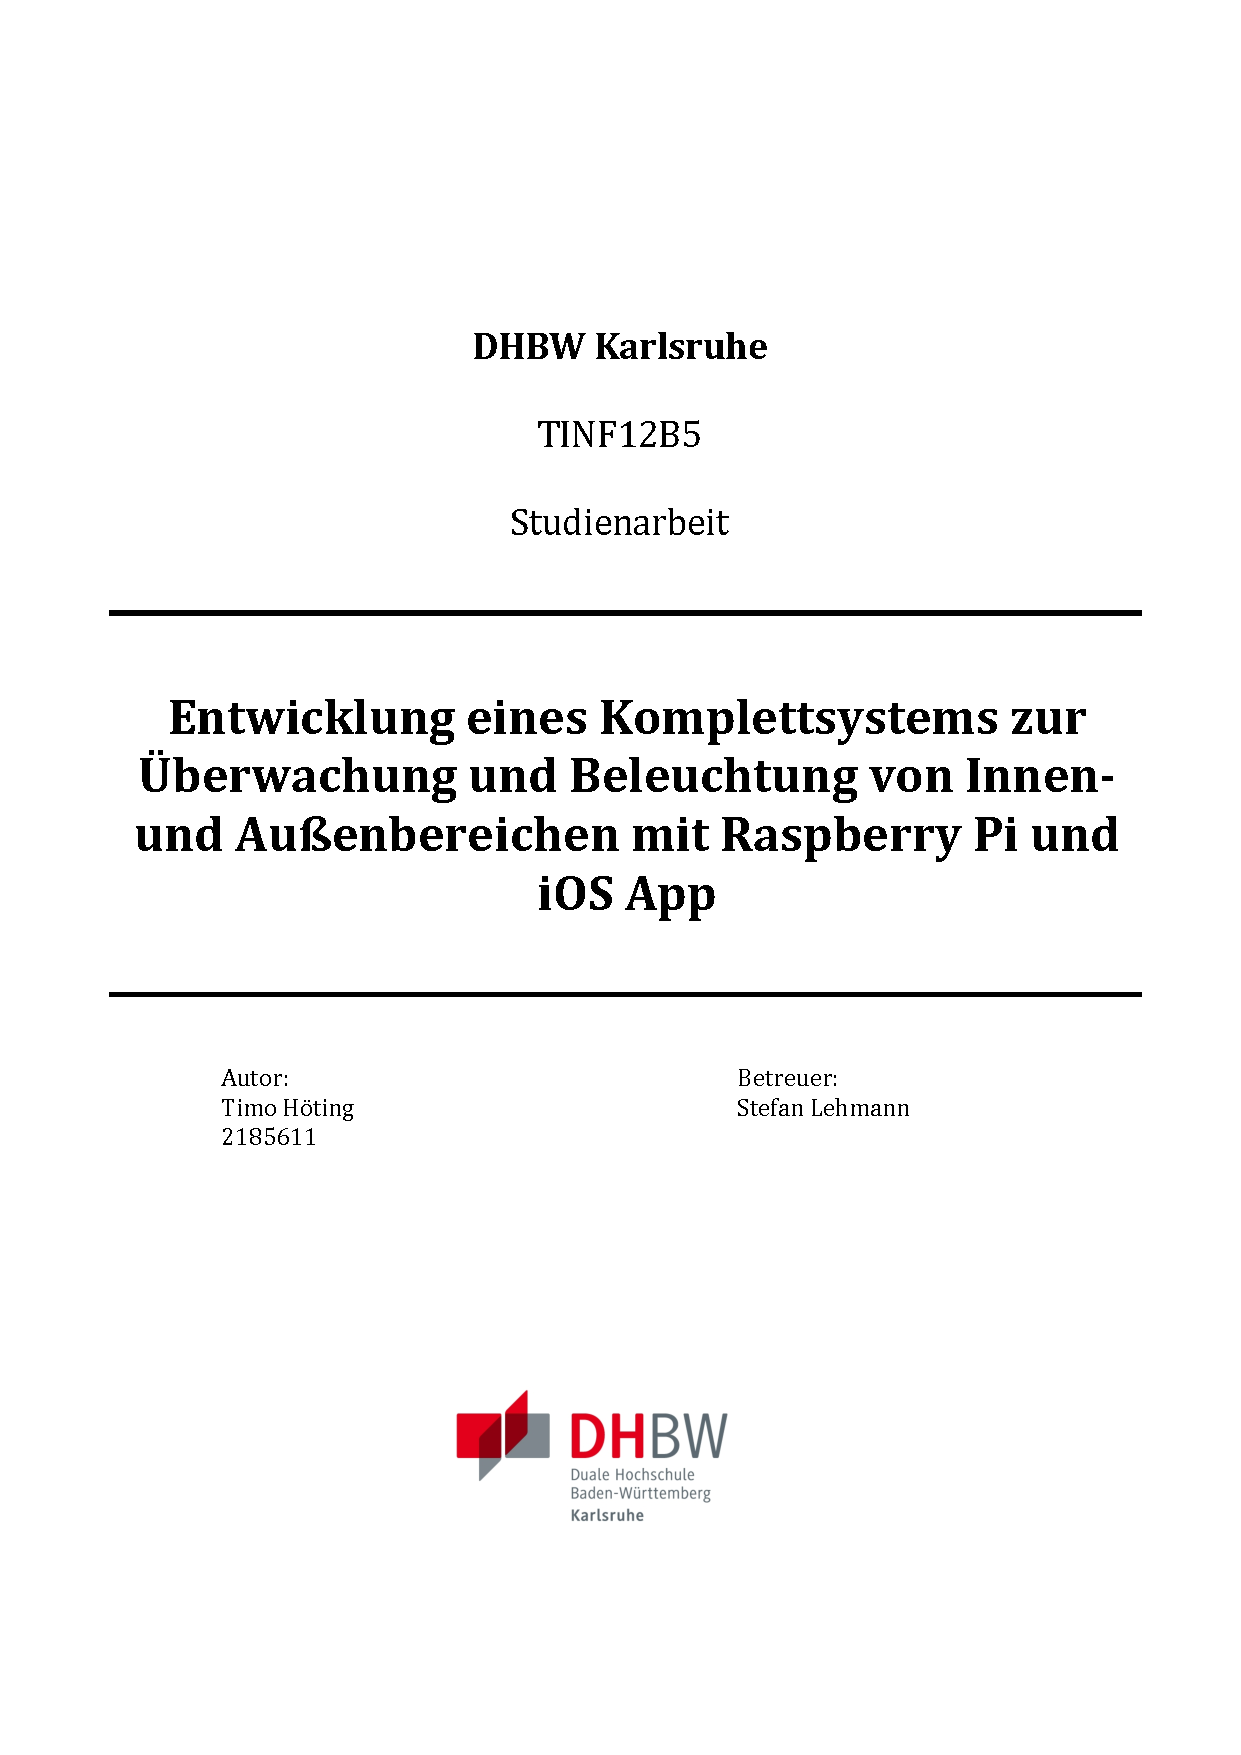
\includegraphics[page={1},width=\paperwidth]{./data/deckblatt.pdf}} \\
\end{figure}
\end{titlepage}
\clearpage
\begin{figure}
\makebox[\textwidth]{\includegraphics[page={2},width=\paperwidth]{./data/deckblatt.pdf}} \\
\end{figure}
\thispagestyle{empty} %Head löschen
 \tableofcontents
\thispagestyle{empty} 
\chapter{Einleitung}
Es soll ein Komplettsystem entwickelt werden, dass sowohl die Überwachung als auch die Steuerung der Beleuchtung von Innen- und Außenbereichen ermöglicht. Das System soll nach Entwicklung universell einsetzbar und leicht konfigurierbar sein. 
\section{Vorwort}
\section{Projektbeschreibung}
Für die Beleuchtung sollen adressierbare LED-Pixel eingesetzt werden, welche möglichst leicht in ihrer Anzahl variiert werden können. Es müssen passende Bauteile und Produkte evaluiert und getestet werden. Diese müssen vom Raspberry Pi ansteuerbar sein.
Die Überwachung findet über eine Kamera statt. Ob diese direkt am Raspberry Pi angeschlossen wird oder sich nur im selben Netzwerk befindet wird im Laufe dieses Projekts erarbeitet. Für die Erkennung von Aktivitäten werden Bewegungsmelder eingesetzt. 
Gesteuert wird das System über einen Raspberry Pi. Von diesem aus werden die LEDs angesteuert, die Sensorsignale ausgewertet und die Befehle der App empfangen.
Um dem User eine einfach Ansteuerung zu ermöglichen wird eine iOS App implementiert. Die hierfür genutzten Sprachen sind Swift und Objective-C. Die Serverfunktionalitäten werden in Python implementiert.
Es gibt drei verschiedene Modi in denen sich das System befinden kann:
\begin{itemize}
\item Beleuchtung wird durch Bewegungsmelder ausgelöst (Reaktion darauf kann vom User definiert werden)
\item Beleuchtung wird manuell vom Benutzer über App gesteuert (Color Chooser, Bereichsauswahl, Leuchteffekte)
\item Bewegungsmelder als Alarmanlage, beim Auslösen wird der Benutzer benachrichtigt und Bild der Kamera als Notifcation auf dem Smartphone angezeigt
\end{itemize}

\section{Teilprojekte}
\begin{itemize}
\item LED-Pixel evaluieren / ansteuern
\item Implementierung der Ansteuerung / des Protokolls (mit den drei verschiedenen Modi)
\item Implementierung der iOS App
\item Vollständige praktische Umsetzung an einem Beispielobjekt
\end{itemize}

\chapter{Hauptteil}
\section{LED-Pixel}
\subsection{Bewertungskriterien}
Die Beleuchtung soll durch einzelne LED-Pixel stattfinden. Ein Pixel bedeutet ein Chip auf dem sowohl die LED und der nötige Treiber sitzt. Für die Evaluierung werden folgende Kriterien gewählt:
\begin{itemize}
\item RGB-Farbraum \\
Die LED muss den gesamten RGB-Farbraum darstellen können. \\
Gewichtung: 5, KO-Kriterium
\item Ansteuerung \\
Da der Raspberry Pi an einigen seiner Pins Pulsweitenmodulation (PWM) bietet, sollten die LED-Pixel ohne extra Hardware ansteuerbar sein. Eine extra Stromversorgung ist aber bei größerer Anzahl an LEDs unabdingbar. \\
Gewichtung: 10
\item Framework \\
Hier wird bewertet ob der jeweilige Hersteller ein fertiges Framework zu seinen Produkten anbietet. \\
Gewichtung: 10
\item Kosten \\
Es werden nur die reinen Produktkosten, also ohne Versand und Zoll, bewertet. \\
Gewichtung: 5
\item Extras \\
An dieser Stelle können mögliche Extras eines Herstellers einfließen. \\
Gewichtung: 5
\end{itemize}

\subsection{Evaluierung}
\begin{itemize}
\item Adafruit, Neopixel \\
https://www.adafruit.com/neopixel \\
LED-Pixel in unzähligen Ausführungen. \\
Sitz der Firma in Tampa, Florida, USA \\
RGB: Chip ist der WS2801, http://www.adafruit.com/datasheets/WS2801.pdf -> Hat volle Abdeckung des RGB-Farbraums \\
Ansteuerung: Findet über PWM-Pin des Raspberry Pi statt. \\
Framework: Framework von Adafruit, welches eine sehr leichte Ansteuerung ermöglichen soll. \\
Kosten: 4 LEDs  7\$, 25 LEDs zusammen  39\$, durch Lieferung aus USA sehr hohe Versandkosten (50\$) \\
Extras: Händler bietet verschiedene Formen und fertige Ketten an. \\
\item LED-Emotion GMBH, LED Streifen \\
http://www.led-emotion.de/de/LED-Streifen-Set.html \\
LED-Streifen, keine Einzelpixel, nur mit Controller, keine API \\
RGB: Voller RGB-Farbraum \\
Ansteuerung: Nur mit Controller  \\
Framework: Keine öffentliche Api, möglicherweise mit Raspberry Pi ansteuerbar  \\
Kosten: 30 LEDs mit Netzteil 79€   \\
Extras: keine
\item DMX4ALL GmbH, MagiarLED Solutions \\
http://www.dmx4all.de/magiar.html \\
Spezialisiert auf DMX-Ansteuerung, keine öffentliche API \\
RGB: VOller RGB-Farbraum \\
Ansteuerung: Wird über DMX-Controller angesteuert, dieser setzt die Signale um. Vermutlich wird auch der WS2801 Chip verwendet. \\
Framework: DMX-Ansteurung über DMX-Controller \\
Kosten: Streifen mit 72 LEDs = 99€ \\
Extras: viele verschiedene Varianten
\item TinkerForge, RGB LED-Pixel \\
https://www.tinkerforge.com/de/shop/accessories/leds.html \\
Scheinen die gleichen wie von Adafruit zu sein, allerdings werden hauptsächlich Controller im Shop angeboten \\
RGB: Chip ist der WS2801, http://www.adafruit.com/datasheets/WS2801.pdf -> Hat volle Abdeckung des RGB-Farbraums \\
Ansteuerung: Nach Anfrage an den Anbieter sollen die LEDs baugleich zu denen von Adafruit sein.  \\
Framework: keins \\
Kosten: 50 LEDs = 59€ \\
Extras: Lieferung aus Deutschland
\end{itemize}
\paragraph{Fazit:}
In der Evaluierung schneiden die Produkte von Adafruit und TinkerForge am besten ab. Für eine erste Teststellung werden die einzelnen LED-Pixel von Adafruit aus den USA bestellt (Neopixel). An diesen soll vor allem die Ansteuerung getestet werden. Falls diese sich bewähren wird für den endgültigen Aufbau auf die LED-Ketten von Tinkerforge zurück gegriffen. 

\subsection{Teststellung}
Für einen ersten Test wurde das in XXX ausgewählte Produkt als einzelne Pixel bestellt. Der Hersteller Adafruit bietet hier 4er-Packungen an. Diese können leicht in eigene Schaltungen eingelötet oder auf Experimentier-Boards gesteckt werden. Bei geringer Anzahl LEDs reicht die 5V-Stromversorgung des Raspberry Pi aus. 
\paragraph{Technische Daten Neopixel:} 
	\begin{itemize}
	\item Maße: 10.2mm x 12.7mm x 2.5mm
	\item Protokollgeschwindigkeit: 800 KHz
	\item Spannung: 5-9VDC  (bei 3,5V gedimmte Helligkeit) 
	\item Strom: 18,5mA / LED, 55mA / Pixel
	\end{itemize}
\paragraph{Framework:}
	\begin{itemize}
	\item RPI\_WS281X (https://github.com/jgarff/rpi\_ws281x)
	\item Sprache: Python
	\item Entwickelt für Raspberry Pi
	\item Vorraussetzung: Python 2.7
	\end{itemize}
\paragraph{Ablauf des Tests:}
\begin{itemize}
\item \textbf{Aufbau der Schaltung}\\
An die einzelnen LED-Pixel wurden Stecker angelötet, damit sie auf das Experimentierboard aufgesteckt werden können. Dann wird die Schaltung nach folgendem Schaltbild verbunden. Wichtig ist, dass beim Raspberry Pi nur Pins verwendet werden können, welche PWM bieten. 
\item \textbf{Installation des Frameworks} 
\begin{lstlisting}[caption = Installation Framework ws281x, language=Python, frame=single, breaklines=true,columns=fullflexible, commentstyle=\color{gray}\upshape, captionpos=b, numbers = left]
wget https://github.com/tdicola/rpi_ws281x/raw/master/python/dist/rpi_ws281x-1.0.0-py2.7-linux-armv6l.egg 
sudo easy_install rpi_ws281x-1.0.0-py2.7-linux-armv6l.egg
\end{lstlisting}
\item \textbf{Testcode}

\begin{lstlisting}[caption = Testcode zur Ansteuerung der LEDs, language=python, frame=single, breaklines=true,columns=fullflexible, commentstyle=\color{gray}\upshape, captionpos=b, numbers = left]
from neopixel import * 
	
LED_COUNT   = 4       # Number of LED pixels. 
LED_PIN     = 18      # GPIO pin connected to the pixels (must support PWM!).
LED_FREQ_HZ = 800000  # LED signal frequency in hertz (usually 800khz)
LED_DMA     = 5       # DMA channel to use for generating signal (try 5)
LED_INVERT  = False   # True to invert the signal (when using NPN)

strip = Adafruit_NeoPixel(LED_COUNT, LED_PIN, LED_FREQ_HZ, LED_DMA, LED_INVERT)

strip.begin()
strip.setPixelColor(0, Color(255, 255, 255))
strip.setPixelColor(1, Color(255, 255, 255))
strip.setPixelColor(2, Color(255, 255, 255))
strip.setPixelColor(3, Color(255, 255, 255))
strip.show()
\end{lstlisting}
\end{itemize}
\subsection{Fazit}
Die einzelnen Pixel sind sehr leicht anzusteuern, unterstützen auch das automatische Abschalten nach einer bestimmten Zeit und haben eine sehr hohe Leuchtkraft. Die Evaluierung hat zu einer guten Produktwahl geführt. In der Endgültigen Projektstellung werden keine einzelnen LEDs eingesetzt, sondern eine fertige Kette des Herstellers. 


\section{Bewegungssensor}
In einem der Modi soll die Beleuchtung durch den Bewegunsmelder ausgelöst werden. Hierfür sind zuverlässige und weitreichende Beweungssensoren notwendig.
\subsection{Bewertungskriterien}
\begin{itemize}
\item \textbf{Ansteuerung}\\
Die Anbindung an den Raspberry Pi soll möglichst leicht realisierbar sein. Wünschenswert ist, dass der Sensor einfach ein High-Signal bei Bewegungserkennung ausgibt. \\
Gewichtung: 5, KO-Kriterium
\item \textbf{Reichweite}\\
Die Reichweite oder Sensivität des Sensors soll ausreichend und regelbar sein.\\
Gewichtung: 3
\item \textbf{Kosten}\\
Es werden nur die reinen Produktkosten, also ohne Versand und Zoll, bewertet. \\
Gewichtung: 1
\item \textbf{Extras}\\
An dieser Stelle können mögliche Extras eines Herstellers einfließen.\\
Gewichtung: 3
\end{itemize}

\subsection{Evaluierung}
\begin{itemize}
\item \textbf{PIR (MOTION) Sensor, Adafruit}\\
Link: http://www.adafruit.com/product/189\\
Ansteuerung: Gibt High-Signal an einem Pin aus.\\
Reichweite: 7m, 120 Grad\\
Kosten: 9,95\$ + Versand aus USA\\
Extras: Kabel inklusive\\
\item \textbf{PIR Infrared Motion Sensor (HC-SR501)}\\
Link: https://www.modmypi.com/pir-motion-sensor\\
Ansteuerung: Gibt High-Signal an einem Pin aus.\\
Reichweite: 5-7m, 100 Grad\\
Kosten: 2,99\$ + Versand aus UK\\
Extras: keine\\
\item \textbf{Infrarot PIR Bewegung Sensor Detektor Modul}\\
Link: http://www.amazon.de/Pyroelectrische-Infrarot-Bewegung-Sensor-Detektor/dp/B008AESDSY/ref=pd\_cp\_ce\_0\\
Ansteuerung: Gibt High-Signal an einem Pin aus.\\
Reichweite: 7m, 100 Grad\\
Kosten: 5 Stück = 7,66€\\
Extras: keine\\
\end{itemize}

\subsection{Fazit}
Die meisten Infarot-Bewegungssensoren sind von der Bauweise nahezu identisch. Die Unterschiede liegen meist nur in der Empfindlichkeit. Da die Reichweite in diesem Fall nicht von großer Bedeutsamkeit ist, kann eigentlich jedes der Produkte bestellt werden. Auf Ebay und Amazon ist die Anzahl angebotener Sensoren nahezu unbegrenzt, es wurde für die Teststellung also die oben evaluierte Variante von Amazon bestellt. 
\subsection{Teststellung}

\section{Python-Server und Protokoll}
\subsection{Protokoll}
\subsection{Framework}
\subsection{Testcode}
\subsection{Implementierung}
\subsection{Klassen und ihre Funktionen}
\subsection{Hashfunktion}

\section{Verschlüsselung}
\subsection{SSL vs. TLS}
\subsection{Vor- und Nachteile TLS}
\subsection{TLS Handshake}
\subsection{Zertifikat und Key}
\subsection{Beispielcode Server}
\subsection{Wireshark Trace}

\section{Kamera}
\subsection{PI-Kamera vs. Netzwerkkamera}
\subsection{Ansteuerung}

\section{iOS App}
\subsection{Konzept}
\subsection{...}
\subsection{...}

\chapter{Praktische Umsetzung}

\chapter{Kostenaufstellung}

\chapter{Fazit}


 \end{document}

 